%%%%%%%%%%%%%%%%%%%%%%%%%%%%%%%%%%%%%%%%%%%%%%%%%%%%%%%%%%%%%%%%%%%%%%%%%%%%%%%%
%2345678901234567890123456789012345678901234567890123456789012345678901234567890
%        1         2         3         4         5         6         7         8

\documentclass[letterpaper, 10 pt, conference]{ieeeconf}  % Comment this line out if you need a4paper

%\documentclass[a4paper, 10pt, conference]{ieeeconf}      % Use this line for a4 paper

\IEEEoverridecommandlockouts                              % This command is only needed if 
                                                          % you want to use the \thanks command

\overrideIEEEmargins                                      % Needed to meet printer requirements.

%In case you encounter the following error:
%Error 1010 The PDF file may be corrupt (unable to open PDF file) OR
%Error 1000 An error occurred while parsing a contents stream. Unable to analyze the PDF file.
%This is a known problem with pdfLaTeX conversion filter. The file cannot be opened with acrobat reader
%Please use one of the alternatives below to circumvent this error by uncommenting one or the other
%\pdfobjcompresslevel=0
%\pdfminorversion=4

% See the \addtolength command later in the file to balance the column lengths
% on the last page of the document

% The following packages can be found on http:\\www.ctan.org
%\usepackage{graphics} % for pdf, bitmapped graphics files
\usepackage{graphicx}
\usepackage{amsmath}
\usepackage{amssymb}
\usepackage{url}
\usepackage{subfigure}
\usepackage{booktabs}
\graphicspath{{./figures/}}

\usepackage{cite}  % converts [1],[2] to [1,2]
\makeatletter
\def\@citex[#1]#2{\leavevmode
\let\@citea\@empty
\@cite{\@for\@citeb:=#2\do
{\@citea\def\@citea{,\penalty\@m\ }%
\edef\@citeb{\expandafter\@firstofone\@citeb\@empty}%
\if@filesw\immediate\write\@auxout{\string\citation{\@citeb}}\fi
\@ifundefined{b@\@citeb}{\hbox{\reset@font\bfseries ?}%
\G@refundefinedtrue
\@latex@warning
{Citation `\@citeb' on page \thepage \space undefined}}%
{\@cite@ofmt{\csname b@\@citeb\endcsname}}}}{#1}}
\makeatother


%\usepackage{dblfloatfix}
%\usepackage{epsfig} % for postscript graphics files
%\usepackage{mathptmx} % assumes new font selection scheme installed
%\usepackage{times} % assumes new font selection scheme installed
%\usepackage{amsmath} % assumes amsmath package installed
%\usepackage{amssymb}  % assumes amsmath package installed

\title{\LARGE \bf
Lectura y Monitoreo Inalámbrico de Sensores y Controladores de un Cuadricóptero utilizando ROS
}


\author{Gabriel Noya Doval$^{1}$, Carlos Serrano Barreto$^{1}$% <-this % stops a space
%\thanks{*This work was not supported by any organization}% <-this % stops a space
\thanks{$^{1}$Grupo de Investigación de Mecatrónica, Universidad Simón Bolívar, Caracas, Venezuela.
        {\tt\small \{13-10982, 13-11349\}@usb.ve}}%
}


\begin{document}

\maketitle
\thispagestyle{empty}
\pagestyle{empty}
%%%%%%%%%%%%%%%%%%%%%%%%%%%%%%%%%%%%%%%%%%%%%%%%%%%%%%%%%%%%%%%%%%%%%%%%%%%%%%%%
\begin{abstract}

Monitorear correctamente los datos provistos por los sensores y el valor de los controladores de los motores de un robot es imprescindible para detectar y corregir posibles fallos. Debido a lo peligroso que puede llegar a ser un cuadricóptero cuando ocurre un error, es necesario contar con un sistema de monitoreo a distancia, para así garantizar la seguridad del desarrollador. Dicho esto, se propone realizar un sistema de monitoreo comunicado por WiFi utilizando \textit{Robotic Operating System} (ROS), que disponga de una interfaz gráfica que permita ver a tiempo real los datos de los sensores y el valor de los controladores de los motores, con el objetivo de asegurar la correcta lectura de los datos y que sea posible ajustar las ganancias de los controladores de una manera segura.
\\
\end{abstract}

\begin{keywords}
Cuadricóptero, controladores, sensores, ROS
\end{keywords}
%%%%%%%%%%%%%%%%%%%%%%%%%%%%%%%%%%%%%%%%%%%%%%%%%%%%%%%%%%%%%%%%%%%%%%%%%%%%%%%%

\section{DESCRIPCIÓN DEL PROYECTO}
Se desea desarrollar e implementar un sistema de lectura y monitoreo inalámbrico de sensores en un cuadricóptero a través de una interfaz gráfica, con el objetivo de verificar su correcto funcionamiento a una distancia prudente para evitar cualquier percance con el robot. Adicionalmente, se desea implementar los controladores PID necesarios para volar de manera estable, además de implementar un sistema para monitorear inalámbricamente los valores de los mismos, con el fín de graficarlos y poder ajustar las ganancias de los mismos, mejorando la calidad del vuelo. Este sistema e interfaz serán realizado utilizando ROS y un cuadricóptero real que se construirá durante la asignatura.


\begin{figure}[htpb]
	\centering
	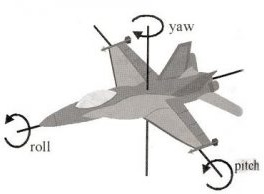
\includegraphics[width=0.99\columnwidth]{angles.jpg}
	\caption{Ángulos medidos y controlados por el giroscopio y por los controladores PID, respectivamente. Imagen tomada de \cite{ypr}.}
	\label{yaw_pitch_roll}
\end{figure}

\section{DESCRIPCIÓN DEL CUADRICÓPTERO}
\subsection{Cuerpo y motores}
El cuadricóptero tiene un cuerpo de fibra de vidrio, modelo S500 de 480mm con PCB de potencia integrado. Contiene cuatro motores EMax 2212 de 980KV, cada uno equipado con una hélice HobbyKing Slowfly 10x4.5. Con esta combinación de motor y hélice, cada motor logra alrededor de 900 gramos de empuje. Para controlar los motores se dispone de cuatro ESC Racerstar de 30A cada uno. 

\subsection{Potencia}
El cuadricóptero es alimentado con una batería LiPo Turnigy de 5000 mAh, contiene tres celdas y posee una tasa de descarga de 20C, es decir, puede otorgar hasta 100 amperios. Esta potencia es distribuida utilizando el \textit{Printed Circuit Board} (PCB) que incluye el cuerpo del drone. Para alimentar las unidades de procesamiento, se cuenta con dos reguladores de voltaje de 5V.

\subsection{Sensores}
Para conocer los ángulos \textit{yaw, pitch} y \textit{roll} del cuadricóptero mostrados en la Figura \ref{yaw_pitch_roll}, se dispone de un giroscopio y acelerómetro MPU6050. Para medir la altura, se dispone del medidor de presión atmosférica MS5611 GY-63 con el que haciendo un simple cálculo, se puede transformar la presión atmosférica en altura sobre el nivel del mar. Adicionalmente, se cuenta con un GPS NEO-6M, una cámara de Raspberry Pi, y un sensor de nivel de batería.

\subsection{Unidades de procesamiento}
Se cuenta con una Raspberry Pi Zero W como unidad de procesamiento principal y con dos Arduino Nano que se encargan del control y lectura de sensores.

\subsection{Comunicación inalámbrica}
El cuadricóptero cuenta con un receptor de radio frecuencia de cinco canales. Además, el Raspberry Pi Zero W posee WiFi integrado, por lo puede ser conectado a internet, haciendo posible controlar y monitorear al robot a través de un computador ajeno.


\section{PROCEDIMIENTO}
El primer paso es instalar un sistema operativo compatible con ROS en el Raspberry Pi. El modelo disponible no es compatible con Ubuntu, por lo que se instalará el sistema operativo Raspbian Stretch \cite{raspbian} y ROS Kinetic. Después de esto, se instalarán los paquetes mencionados en la Sección \ref{paquetes} y se probará que ROS funcione de manera remota al comunicarse con un computador en la misma red. A continuación, se programará la lectura de los sensores en Arduino, se probarán y se publicarán sus datos como tópicos en ROS. Una vez terminada la programación de la lectura de todos los sensores esenciales para el vuelo, se procederá a programar la interfaz gráfica utilizando una aplicación web o una aplicación creada con Node.js y Electron conectada con ROS.

Una vez sea posible monitorear los sensores de una manera segura, se procederá a implementar los controladores PID para controlar los ángulos \textit{yaw, pitch} y \textit{roll}. Luego, se publicarán las salidas de los controladores para poder ser graficadas y ajustadas.


\subsection{DIAGRAMA DE BLOQUES}
Bla bla bla bla Bla bla bla bla Bla bla bla bla Bla bla bla bla
Bla bla bla bla Bla bla bla bla Bla bla bla bla Bla bla bla bla
Bla bla bla bla Bla bla bla bla Bla bla bla bla Bla bla bla bla
Bla bla bla bla Bla bla bla bla Bla bla bla bla Bla bla bla bla
Bla bla bla bla Bla bla bla bla Bla bla bla bla Bla bla bla bla
Bla bla bla bla Bla bla bla bla Bla bla bla bla Bla bla bla bla

\subsection{PAQUETES}
\label{paquetes}
Se utilizarán los paquetes \textbf{rosserial} \cite{rosserial} y \textbf{rosserial\textunderscore arduino} \cite{rosserialarduino} para crear un nodo en cada Arduino y que puedan publicar tópicos a través del puerto serial que contengan la información de interés.

Para comunicar ROS con la aplicación donde se desarrollará la interfaz gráfica, se utilizará el paquete \textbf{rosbridge\textunderscore suite} \cite{rosbridge}, que permite la comunicación entre ROS y otros programa a través de una API JSON.

\section{CRONOGRAMA DE ACTIVIDADES}
Bla bla bla bla Bla bla bla bla Bla bla bla bla Bla bla bla bla
Bla bla bla bla Bla bla bla bla Bla bla bla bla Bla bla bla bla
Bla bla bla bla Bla bla bla bla Bla bla bla bla Bla bla bla bla
Bla bla bla bla Bla bla bla bla Bla bla bla bla Bla bla bla bla
Bla bla bla bla Bla bla bla bla Bla bla bla bla Bla bla bla bla
Bla bla bla bla Bla bla bla bla Bla bla bla bla Bla bla bla bla


%\addtolength{\textheight}{-7cm}   % This command serves to balance the column lengths
                                  % on the last page of the document manually. It shortens
                                  % the textheight of the last page by a suitable amount.
                                  % This command does not take effect until the next page
                                  % so it should come on the page before the last. Make
                                  % sure that you do not shorten the textheight too much.

%%%%%%%%%%%%%%%%%%%%%%%%%%%%%%%%%%%%%%%%%%%%%%%%%%%%%%%%%%%%%%%%%%%%%%%%%%%%%%%%
%\section*{APPENDIX}
%

%%%%%%%%%%%%%%%%%%%%%%%%%%%%%%%%%%%%%%%%%%%%%%%%%%%%%%%%%%%%%%%%%%%%%%%%%%%%%%%%

%\begin{thebibliography}{99}
%\item 
%\end{thebibliography}


\bibliography{references}
\bibliographystyle{ieeetr}

\end{document}
